\chapter{Physical Network Design}

\section{Devices}
\subsection{Workstations}
It is assumed that all workstations in use have been bought over from the old branch to reduce on cost. The only upgrade that would have to be made to each workstation is the installation of an SFP+ network adaptor. The recommended PCI expansion card is the \emph{ASUS 10GbE SFP+ PCIe 3.0 Network Adapter}. This recommendation is due to high reviews and a reputable manufacturer.
\subsection{Servers}
Any servers needed in the network such as email, DNS or vpn will be generic Linux based draws stored in the server room. Inside the network these servers will be placed within the DMZ area.
\subsection{Wireless Access Points (WAP)}
The Cisco Catalyst 9136 WAP has been chosen for its ability to use WiFi 6, further future-proofing our network solution.
\subsection{Media Converter}
When applicable for use the TP-Link MC220L media converter will be used to allow for use of copper cabling. An example of this use case would be the connection from switch to WAP as the WAP does not have an SFP+ port.
\subsection{Layer 3 Switch}
\subsubsection{Chassis - C4506-E}
It has been assumed that this is a switch that has been bought over from the old building to save on costs. It is an older model that is no longer sold but is going to be supported by Cisco until 2025 \parencite{cisco-4506}.
\subsubsection{Line Card - WS-X4712-SFP+E5}
This line card has been chosen because it can handle the speed of the network while being able to fit multiple in the chosen layer 3 chassis.
\begin{table}[H]
    \centering
    \begin{tabular}{|cccc|}
    \hline
    \multicolumn{1}{|c|}{SKU} & \multicolumn{1}{c|}{Ports} & \multicolumn{1}{c|}{Speed} & Connector \\ \hline
    WS-X4712-SFP+E5           & 12                         & 10GBASE-R                  & SFP+/SFP  \\ \hline
    \end{tabular}
    \caption{Specifications for the WS-X4712-SFP+E5 line card \parencite{layer3-lc-datasheet}}
\end{table}
\subsection{Layer 2 Switch}
The layer 2 switches will be housed in the patch panels situated on each floor. They will handle the switching of packets between the end devices and the distribution layer.
\subsubsection{Chassis - C9404R}
This chassis has been chosen as it is the correct size needed to fit two supervisor cards and two line cards. This allows for the correct number of ports as well as additional for company expansion. Going any larger would not be beneficial and cost more. 
\subsubsection{Line Card - C9400-LC-48XS}
This line card has been chosen for the access layer switch as we can fit two of them in the chosen chassis. This will provide enough ports to cover the existing devices on each floor as well as any new devices bought in due to expansion.
\begin{table}[H]
    \centering
    \begin{tabular}{|ccccc|}
    \hline
    \multicolumn{1}{|c|}{SKU} & \multicolumn{1}{c|}{Ports} & \multicolumn{1}{c|}{Connector} & \multicolumn{1}{c|}{Speed} & Total Needed \\ \hline
    C9400-LC-48XS             & 48                         & SFP/SFP+                       & 1/10Gbps                   & 2            \\ \hline
    \end{tabular}
    \caption{Specifications for the c9400-LC-48XS linecard \parencite{layer2-lc-datasheet}.}
\end{table}
\subsection{Router}
Cisco 4000 Series Integrated Services Router
\subsection{Firewall- Cisco Firepower 4125}

\section{Wiring}
A full fiber solution will be employed for this network to account for future proofing and to reduce noise on the network. Copper based ethernet may be used when fiber is not an option for that device.
\subsection{Multi-mode Fiber - OM4}
The current network will be 10GBASE-SR, using OM4 fiber cables. Using OM4 fiber will give us options to expand to 40GBASE-SR or 100GBASE-SR in future also.
As the solution planned for this building is mostly copperless, OM4 cables will run between all three layers of our network model.
While the distance of 400m at 10Gbps for OM4 is overkill for a 7 story building, the allowance for higher distances at higher speeds (100m at 100Gbps) will be good for future-proofing our solution.
The cost of fiber has been decreasing steadily over the past years, due to this there will not be much of a difference between the cost of copper and fiber ethernet solutions. The only additional cost over a copper solution will be the installation of fiber network adaptors in workstation PCs.
\begin{table}[H]
    \centering
    \begin{tabular}{|ccccc|}
    \hline
    \multicolumn{1}{|c|}{\multirow{2}{*}{Designation}} & \multicolumn{4}{c|}{Distance (m)}                                                                                \\ \cline{2-5} 
    \multicolumn{1}{|c|}{}                             & \multicolumn{1}{c|}{1000BASE-SX} & \multicolumn{1}{c|}{10GBASE-SR} & \multicolumn{1}{c|}{40GBASE-SR4} & 100GBASE-SR10 \\ \hline
    OM1                                                & 275                            & 33                              & N/A                             & N/A         \\ \hline
    OM2                                                & 550                            & 82                              & N/A                             & N/A         \\ \hline
    OM3                                                & N/A                            & 300                             & 100                             & 100         \\ \hline
    OM4                                                & N/A                            & 550                             & 150                             & 150         \\ \hline
    OM5                                                & N/A                            & 550                             & 150                             & 150         \\ \hline
    \end{tabular}
    \caption{Table of distances for Multi-mode Fiber cables \parencite{mm-fiber-stats}.}
    \label{tab:fiber_distance}
\end{table}
\subsection{Copper Ethernet - CAT5e}

\section{Uninterruptible Power Supply - 2x SRV10KIL with 4x SRV240BP-9A}
Due to the risk of earthquakes and other natural disasters present in Tokyo, Uninterruptible Power Supplies are recommended for this network installation. When the mains power is interrupted these UPS units will keep the infrastructure online for enough time to initiate graceful shutdowns or wait for mains power to come back.
The addition of extra battery packs will allow for extended runtime when no mains power is being supplied.
\begin{table}[H]
    \centering
    \begin{tabular}{|cccc|}
    \hline
    \multicolumn{1}{|c|}{SKU} & \multicolumn{1}{c|}{Output capacity} & \multicolumn{1}{c|}{Runtime at max load} & Total Needed \\ \hline
    SRV10KIL                  & 10000W                               & 2m 32s                                   & 2            \\ \hline
    \end{tabular}
    \caption{Specifications for SRV10KIL \parencite{ups-specs}}
\end{table}
\begin{table}[H]
    \begin{tabular}{|cccc|}
    \hline
    \multicolumn{1}{|c|}{SKU} & \multicolumn{1}{c|}{Output capacity} & \multicolumn{1}{c|}{Runtime at max load} & Total Needed \\ \hline
    SRV240BP-9A               & 10000W                               & 2m 32s                                   & 4            \\ \hline
    \end{tabular}
    \caption{Specifications for SRV240BP-9A \parencite{bp-specs}}
\end{table}
\subsection{Patch Panels}
Patch panels will be placed on each floor to house access section L2 switches. This allows us to create several points of failure, as opposed to a single point of failure of storing all switches in the server room.
\section{Device Placement}
The placement of devices in the offices and in the server room is outlined in the below sections.
\subsection{Ground Floor}
\begin{figure}[H]
    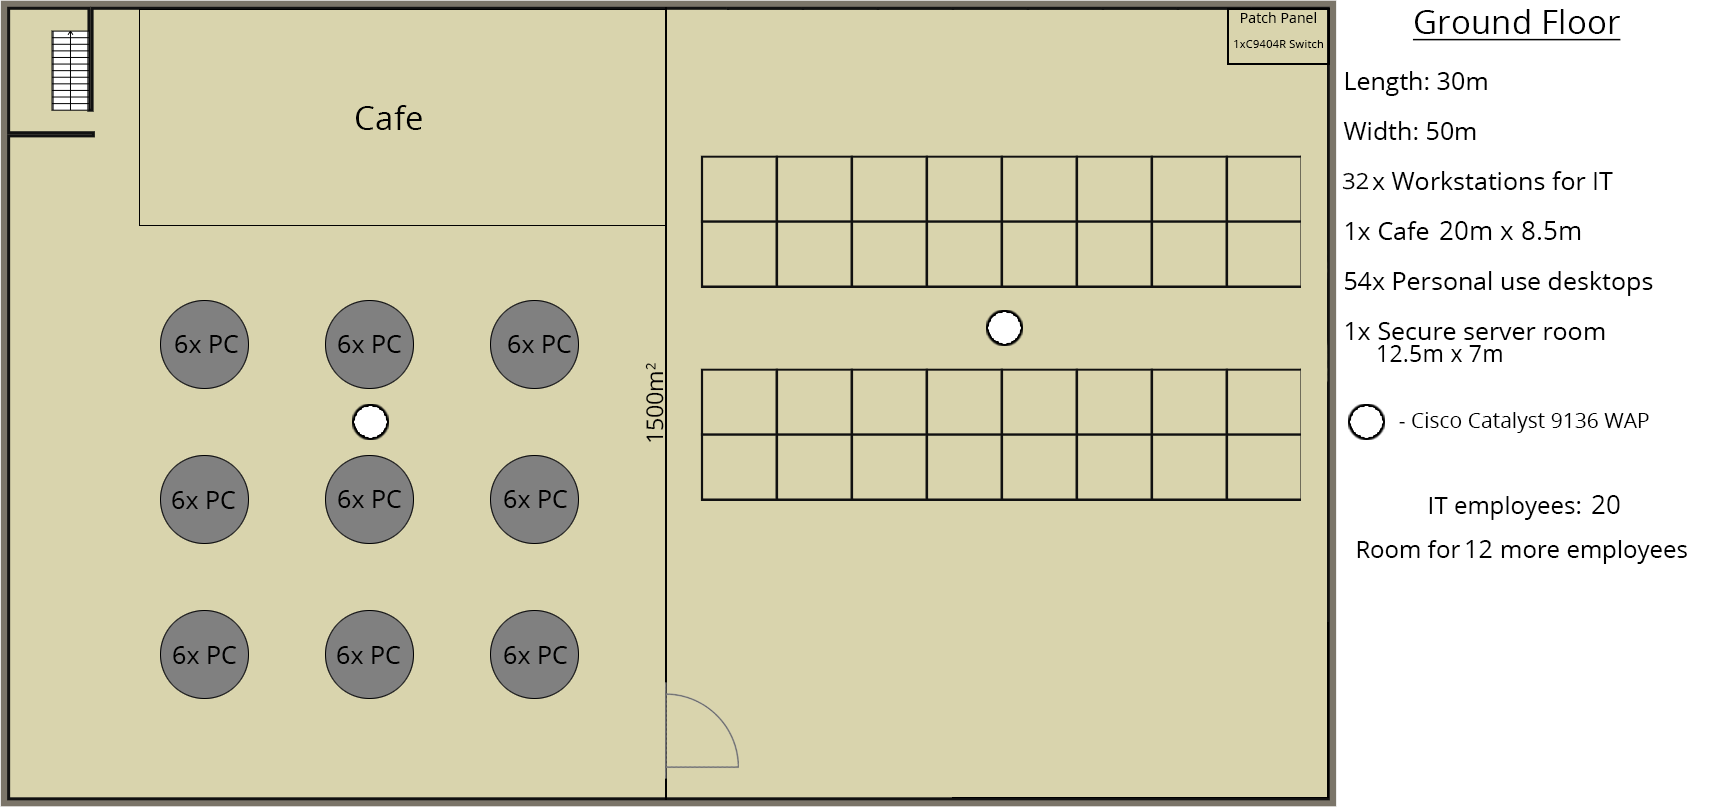
\includegraphics[width=15cm]{Figures/ground.png}
    \caption{Ground floor plan}
    \label{fig:ground_floor}
\end{figure}
\subsection{1st Floor}
\begin{figure}[H]
    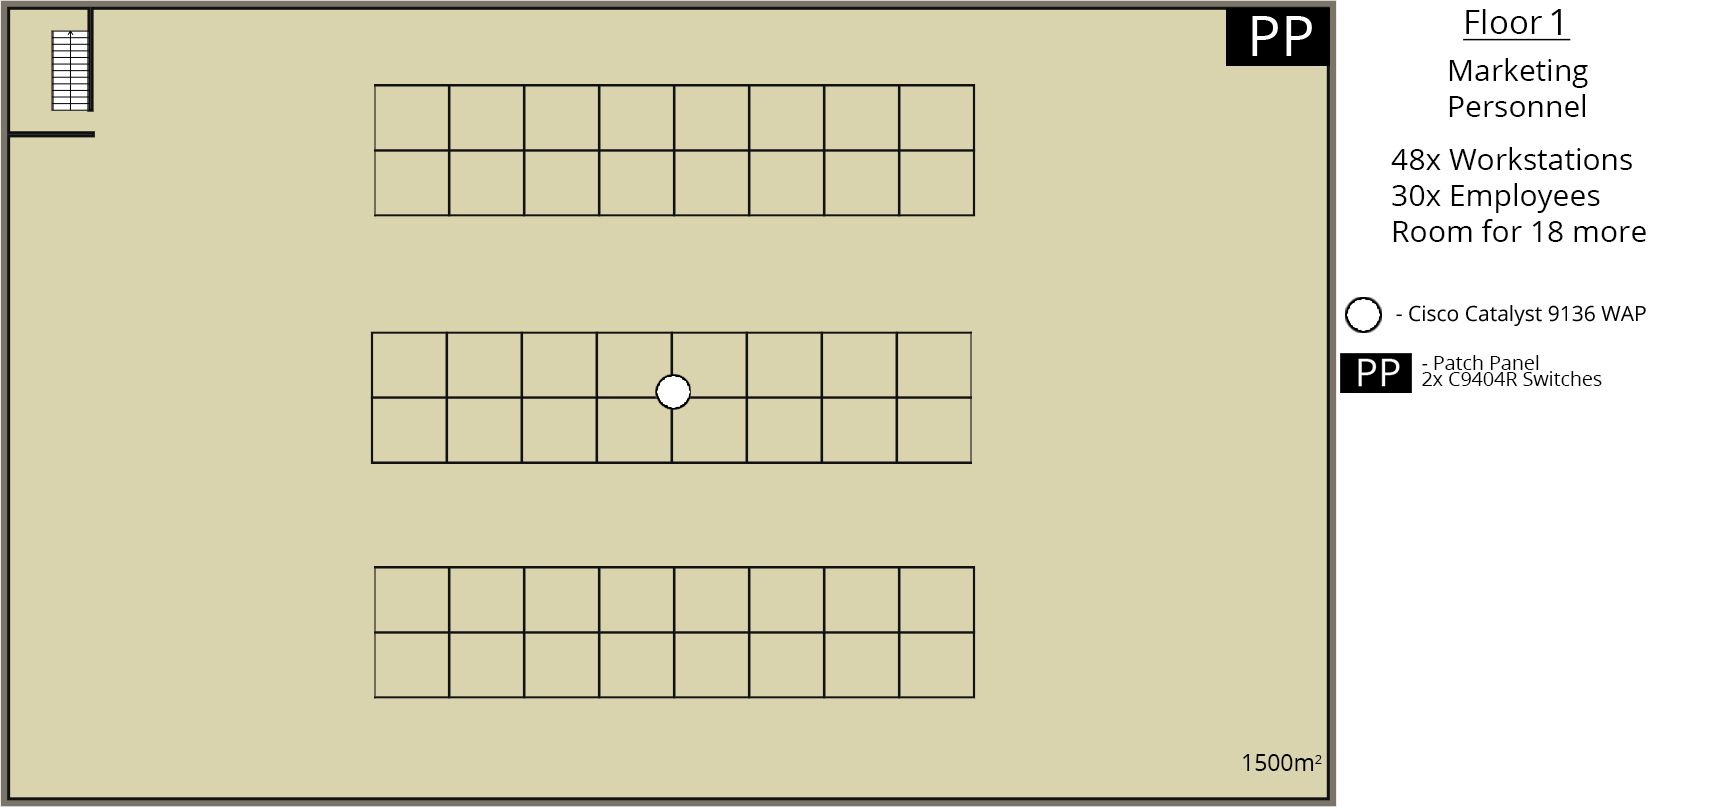
\includegraphics[width=15cm]{Figures/1st-floor.png}
    \caption{1st floor plan}
    \label{fig:1st_floor}
\end{figure}
\subsection{2nd Floor}
\begin{figure}[H]
    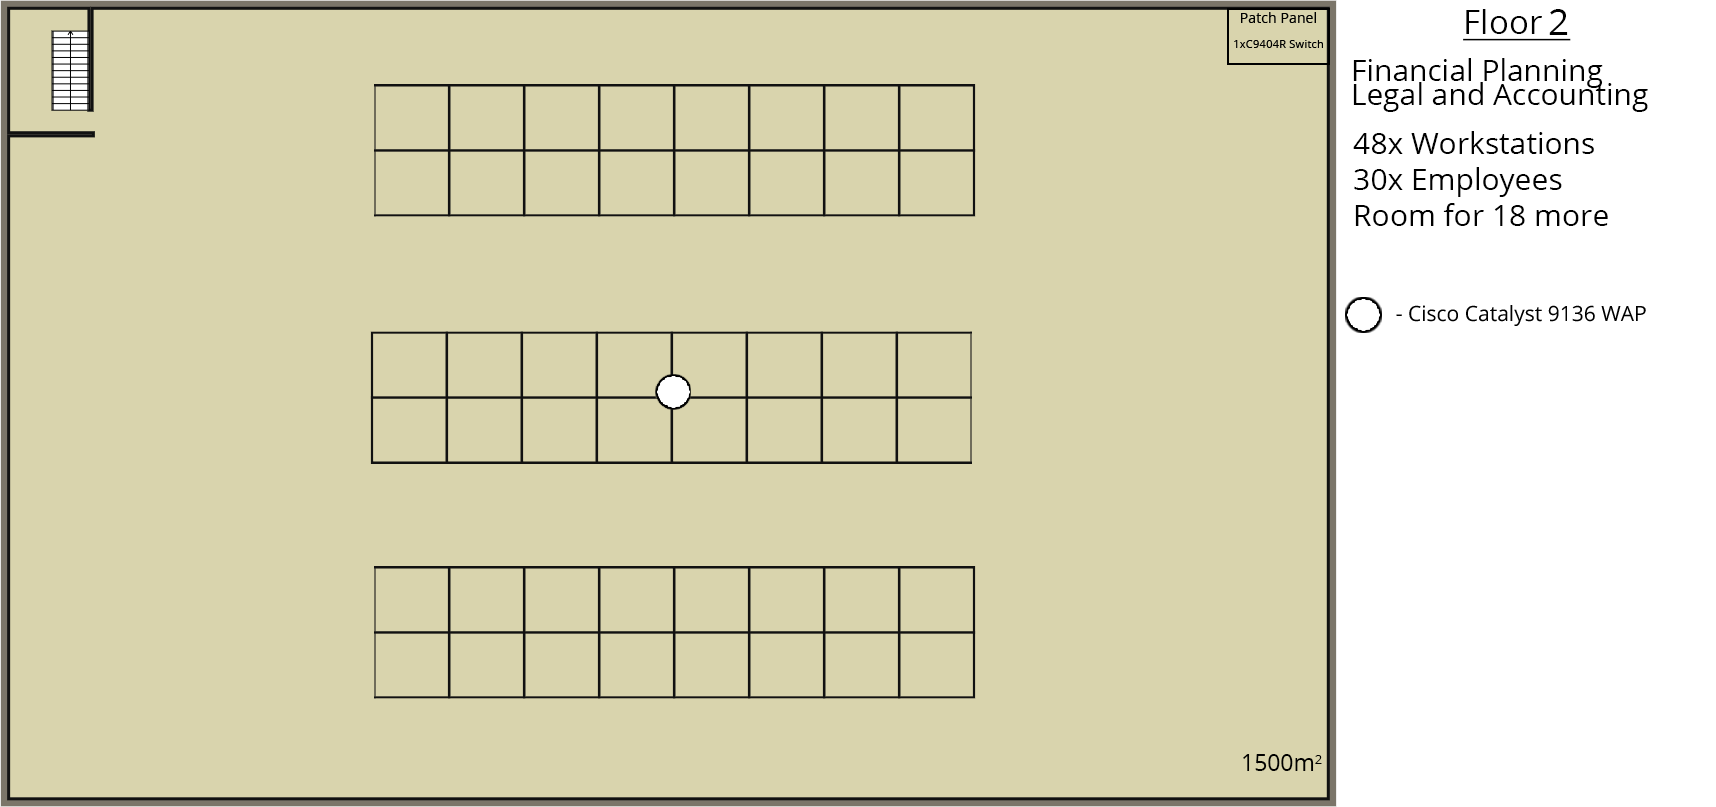
\includegraphics[width=15cm]{Figures/2nd-floor.png}
    \caption{2nd floor plan}
    \label{fig:2nd_floor}
\end{figure}
\subsection{3rd Floor}
\begin{figure}[H]
    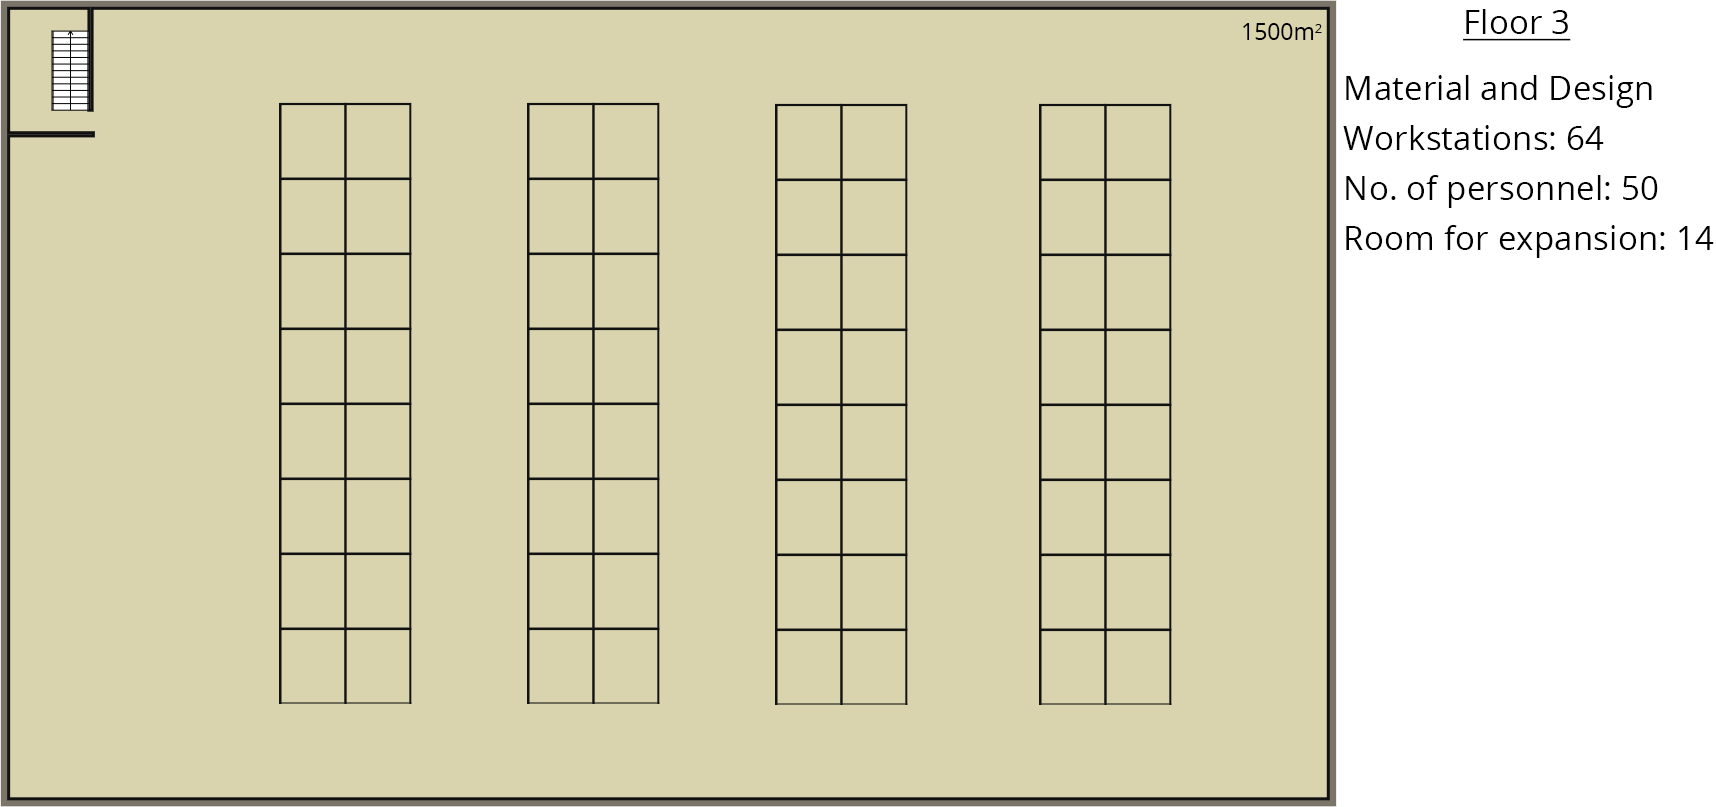
\includegraphics[width=15cm]{Figures/3rd-Floor.png}
    \caption{3rd floor plan}
    \label{fig:3rd_floor}
\end{figure}
\subsection{4th Floor}
\begin{figure}[H]
    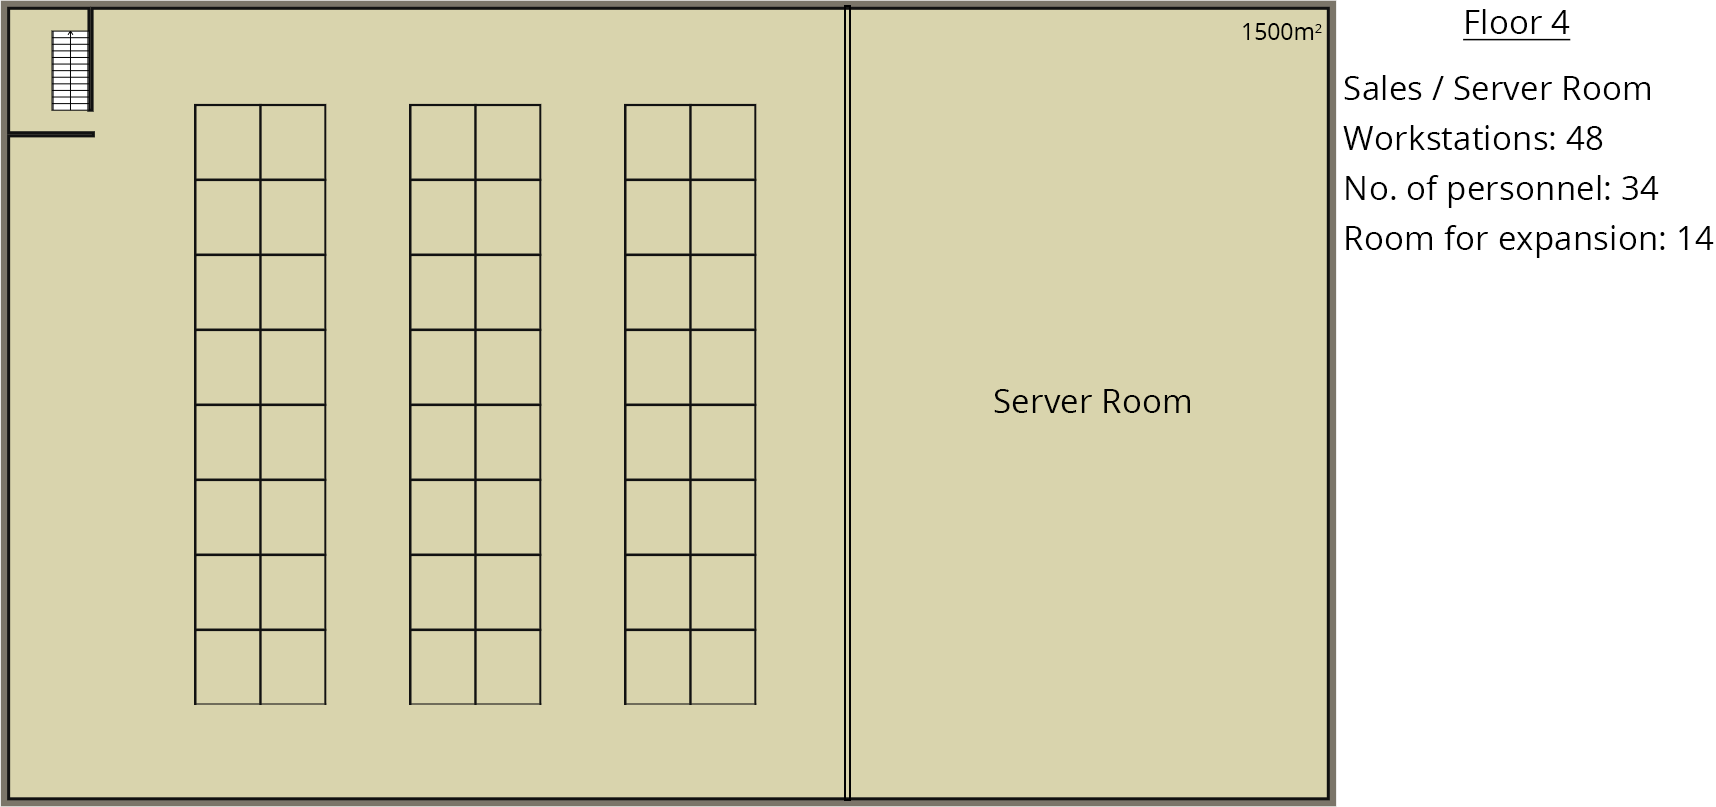
\includegraphics[width=15cm]{Figures/4th-Floor.png}
    \caption{4th floor plan}
    \label{fig:4th_floor}
\end{figure}
Explain why server room here
\subsection{5th Floor}
\begin{figure}[H]
    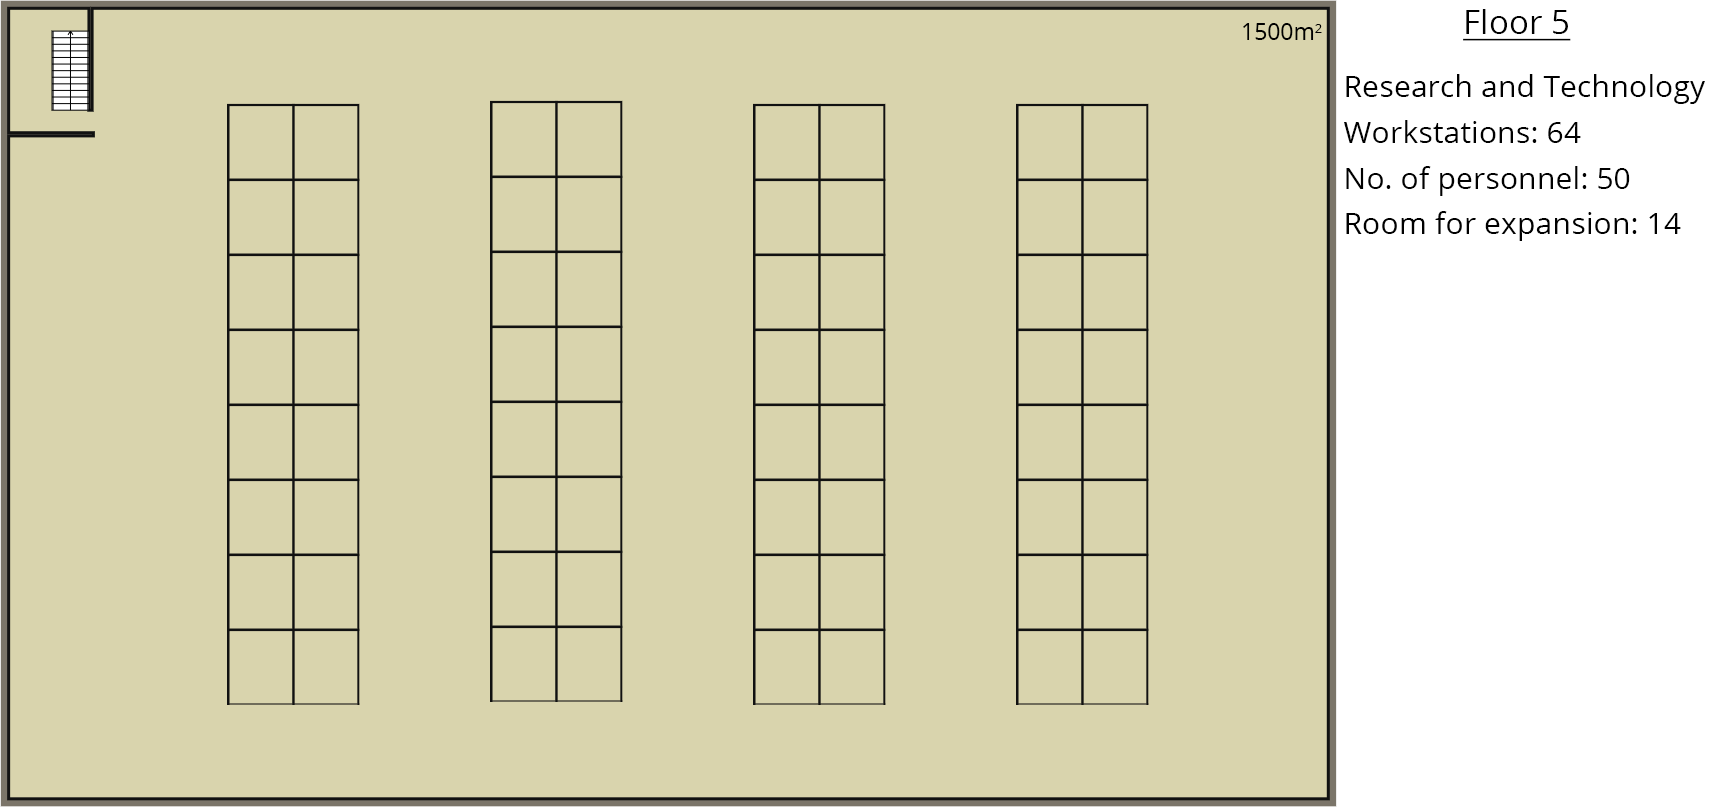
\includegraphics[width=15cm]{Figures/5th-Floor.png}
    \caption{5th floor plan}
    \label{fig:5th_floor}
\end{figure}
\subsection{6th Floor}
\begin{figure}[H]
    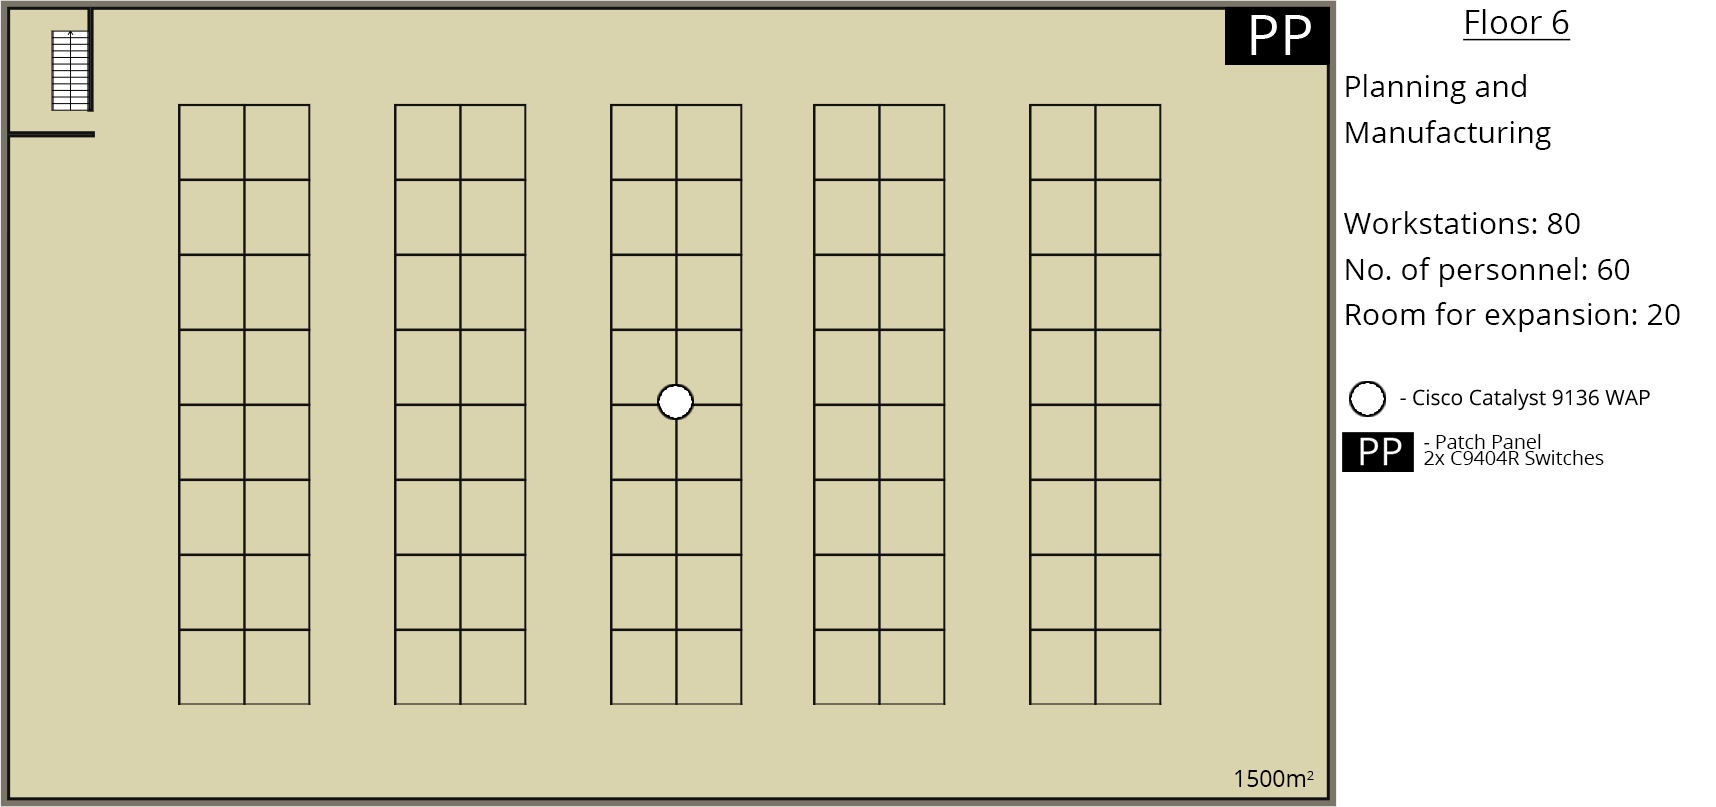
\includegraphics[width=15cm]{Figures/6th-Floor.png}
    \caption{6th floor plan}
    \label{fig:6th_floor}
\end{figure}
\subsection{7th Floor}
\begin{figure}[H]
    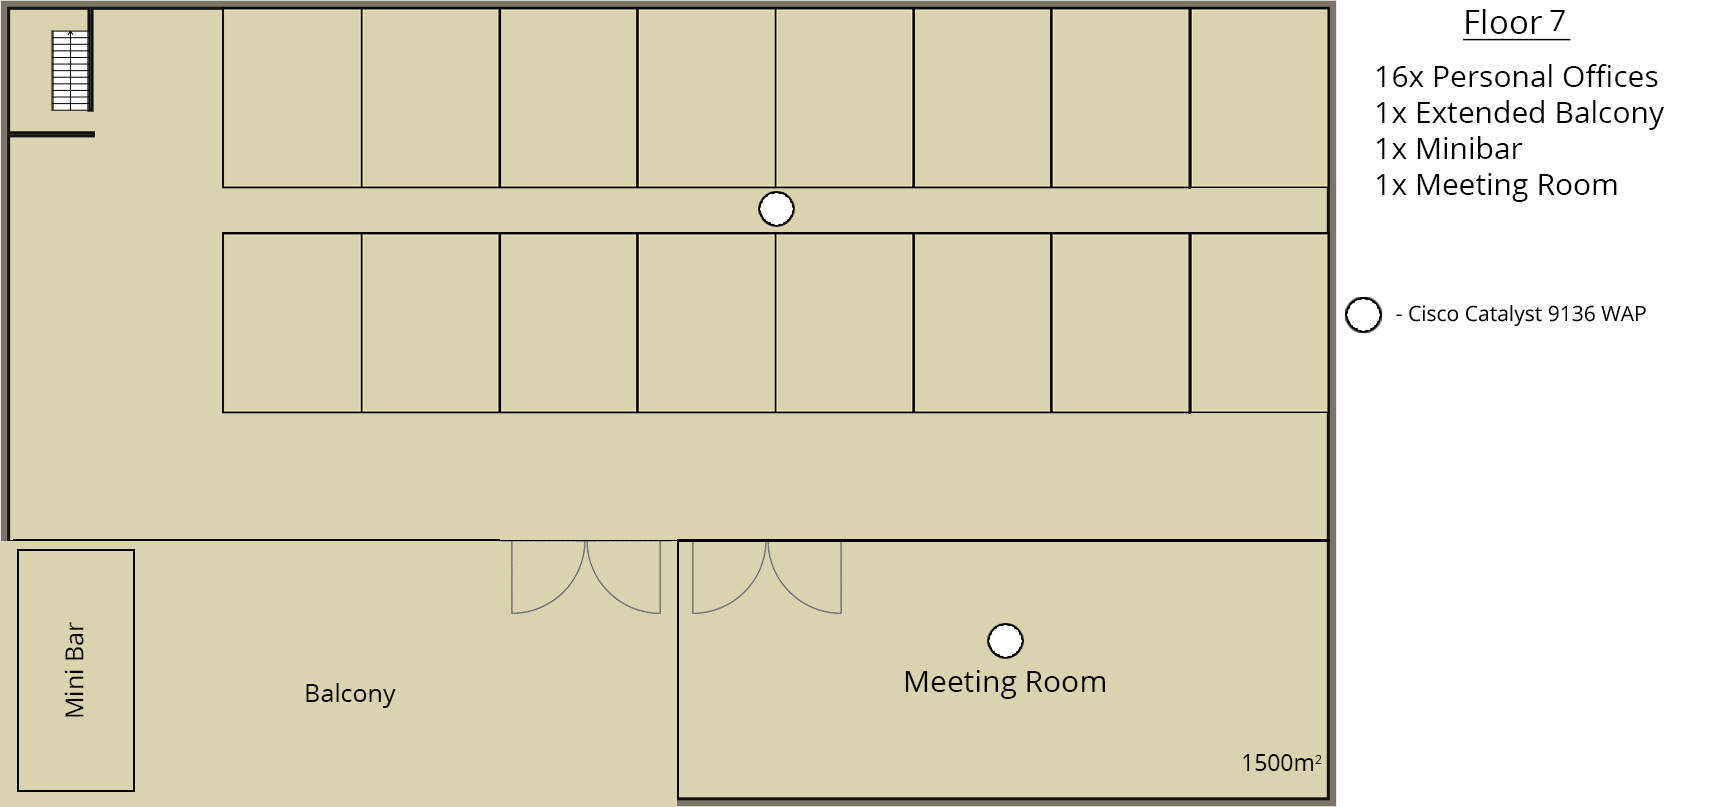
\includegraphics[width=15cm]{Figures/7th-floor.png}
    \caption{7th floor plan}
    \label{fig:7th_floor}
\end{figure}
\subsection{Server Room}
% \begin{figure}
%     \centering
%     \includegraphics[width=15cm]{Figures/}
%     \caption{Server racks diagram configured in Cisco PacketTracer}
%     \label{fig:}
% \end{figure}